\documentclass[14pt]{extarticle}
\usepackage[]{cite}
\usepackage{cmap}
\usepackage[T2A]{fontenc}
\usepackage[utf8]{inputenc}
\usepackage[english, russian]{babel}
\usepackage{amsmath, amsfonts,amssymb,mathrsfs}
\usepackage{graphicx, epsfig}
\usepackage{subfig}
\usepackage{color}

\usepackage{wrapfig}
\usepackage{float}
\usepackage{subfloat}
\usepackage{caption}
\usepackage{multirow}
\graphicspath{{../pics/}}

\newcommand\argmin{\mathop{\arg\min}}
\newcommand{\T}{^{\text{\tiny\sffamily\upshape\mdseries T}}}
\newcommand{\hchi}{\hat{\boldsymbol{\chi}}}
\newcommand{\hphi}{\hat{\boldsymbol{\varphi}}}
\newcommand{\bchi}{\boldsymbol{\chi}}
\newcommand{\A}{\mathcal{A}}
\newcommand{\B}{\mathcal{B}}
\newcommand{\x}{\mathbf{x}}
\newcommand{\hx}{\hat{x}}
\newcommand{\hy}{\hat{y}}
\newcommand{\M}{\mathcal{M}}
\newcommand{\N}{\mathcal{N}}
\newcommand{\R}{\mathbb{R}}
\newcommand{\p}{p(\cdot)}
\newcommand{\q}{q(\cdot)}
\newcommand{\uu}{\mathbf{u}}
\newcommand{\vv}{\mathbf{v}}


\renewcommand{\baselinestretch}{1}


\newtheorem{Th}{Теорема}
\newtheorem{Def}{Определение}
\newenvironment{Proof} % имя окружения
    {\par\noindent{\bf Доказательство.}} % команды для \begin
    {\hfill$\scriptstyle\blacksquare$} % команды для \end
\newtheorem{Assumption}{Предположение}
\newtheorem{Corollary}{Следствие}

\textheight=22cm % высота текста
\textwidth=16cm % ширина текста
\oddsidemargin=0pt % отступ от левого края
\topmargin=-1.5cm % отступ от верхнего края
\parindent=24pt % абзацный отступ
\parskip=5pt % интервал между абзацами
\tolerance=2000 % терпимость к "жидким" строкам
\flushbottom % выравнивание высоты страниц

%\graphicspath{ {fig/} }



\begin{document}

\thispagestyle{empty}
\begin{center}
    \sc
        ФГАОУВО «Московский физико-технический институт \rm{(национальный исследовательский университет)}»\\
        Физтех-школа прикладной математики и информатики\\
        Кафедра <<Интеллектуальные системы>>\\
        при Вычислительном центре им. А. А. Дородницына РАН\\[35mm]
    \rm\large
        Северилов Павел Андреевич\\[10mm]
    \bf\Large
		Оценка качества прогнозирования структуры белка с использованием графовых свёрточных нейронных сетей\\[10mm]
    \rm\normalsize
        03.03.01 -- Прикладные математика и физика\\[10mm]
    \sc
        Выпускная квалификационная работа бакалавра\\[10mm]
\end{center}
\hfill\parbox{80mm}{
    \begin{flushleft}
    \bf
        Научный руководитель:\\
    \rm
        д.~ф.-м.~н. Стрижов Вадим Викторович\\[3cm]
    \end{flushleft}
}
\begin{center}
    Москва\\
    2020
\end{center}


\newpage
\tableofcontents
\newpage

\begin{abstract}
  Решается задача оценки качества (QA -- Quality Assessment) прогнозирования белковых структур. В работе показывается применимость к рассматриваемой задаче графовых свёрточных нейронных сетей, основанных на спектральной теории. Описание белковых структур представляется в виде графов. Спектральная теория графов определяет свёртку в нейронных сетях. Нейросеть в работе получает на вход матрицы координат атомов и матрицы смежности смоделированных белковых структур. Она предсказывает близость смоделированной и реальной структуры белка в виде $\text{CAD}_\text{score}$. Нейросеть обучается на наборах данных CASP7-CASP11 и тестируется на данных CASP12. На CASP12 достигается уровень ошибки MSE равный 0.051. Дополнительный анализ корреляционных коэффициентов Пирсона и Спирмена подтверждает применимость метода для различных белковых структур. Эксперименты в данной работе показывают новые направления в задаче QA.

  \bigskip
  \textbf{Ключевые слова}: \emph{белковые структуры, графы, графовые нейронные сети, свёрточные нейронные сети, спектральные свёртки.}
\end{abstract}

\newpage

%%%%%%%%%%%%%%%%%%%%%%%%%%%%%%%%%%%%%%%%%%%%%%%%%%%%%%%%%%%%%%%%%%%%%%%%%%%%%%%%%%%%%%%%%%%%%%%%%%%%%%%%%%%%%%%%%%%%%%%%%%%%%%%%%%
%\section*{Введение}
%\addcontentsline{toc}{section}{\protect\numberline{}Введение}

	\section{Введение}
	\label{sec:intro}
	
	Белки являются наиболее универсальными макромолекулами в живых системах и выполняют важнейшие функции практически во всех биологических процессах~\cite{berg2002biochemistry}. (?Понимание белковых структур и выполняемых задач помогают контролировать биологические процессы.?)%Белки спонтанным образом принимают форму в различных средах [?] --  
	Форма белковой структуры определяет выполняемые ей функции (?её функционал?)~\cite{berg2002biochemistry}. Но из имеющихся последовательностей аминокислот в белке трудно определить, в какую форму сворачивается структура. Идентификация структуры занимает большое количество времени и ресурсов, к тому же, не всегда возможна. 

Каждые два года проводятся соревнования Critical Assessment of protein Structure Prediction (CASP~\cite{CASP}) по решению задачи предсказания структуры. 	Вычислительные методы, которые её решают состоят из двух этапов: генерация конформаций белка из их аминокислотных последовательностей и оценивание качества предсказания. В данной работе рассматривается только второй этап.
\begin{figure}[H]
	\centering
	\subfloat[True T0861]{\label{fig:edge-a}
		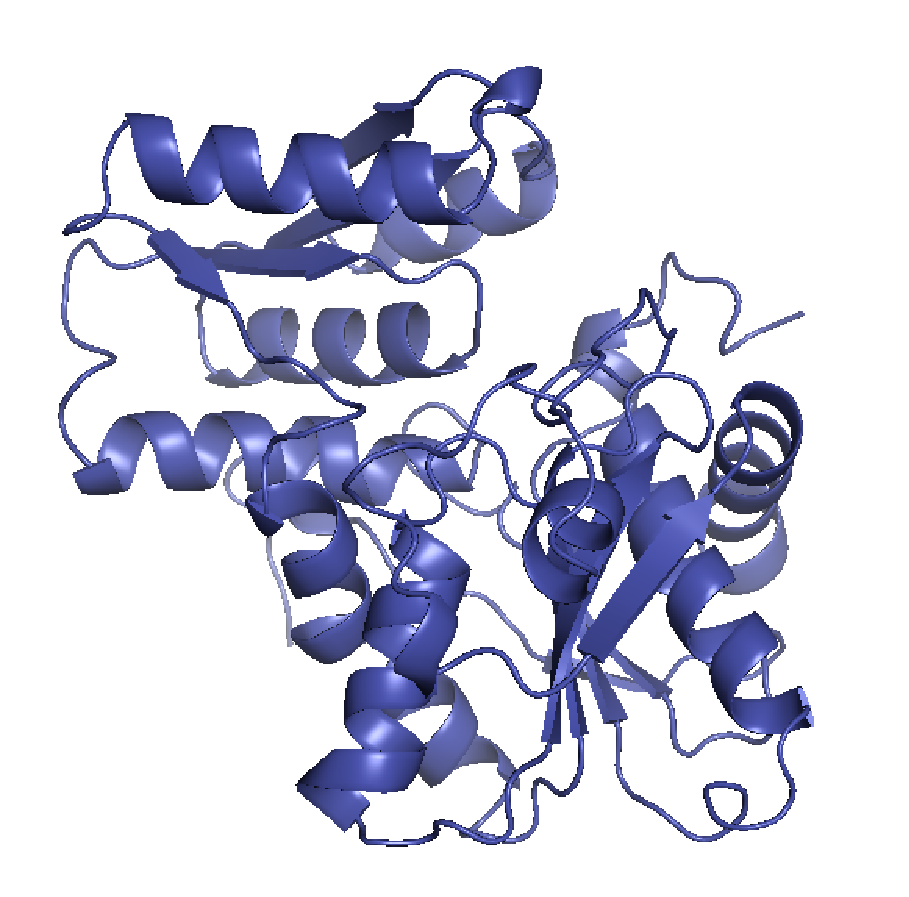
\includegraphics[scale=0.25]{target_T0861.pdf}}
	\subfloat[Predicted Atome2\_CBS\_TS4]{\label{fig:edge-b}
		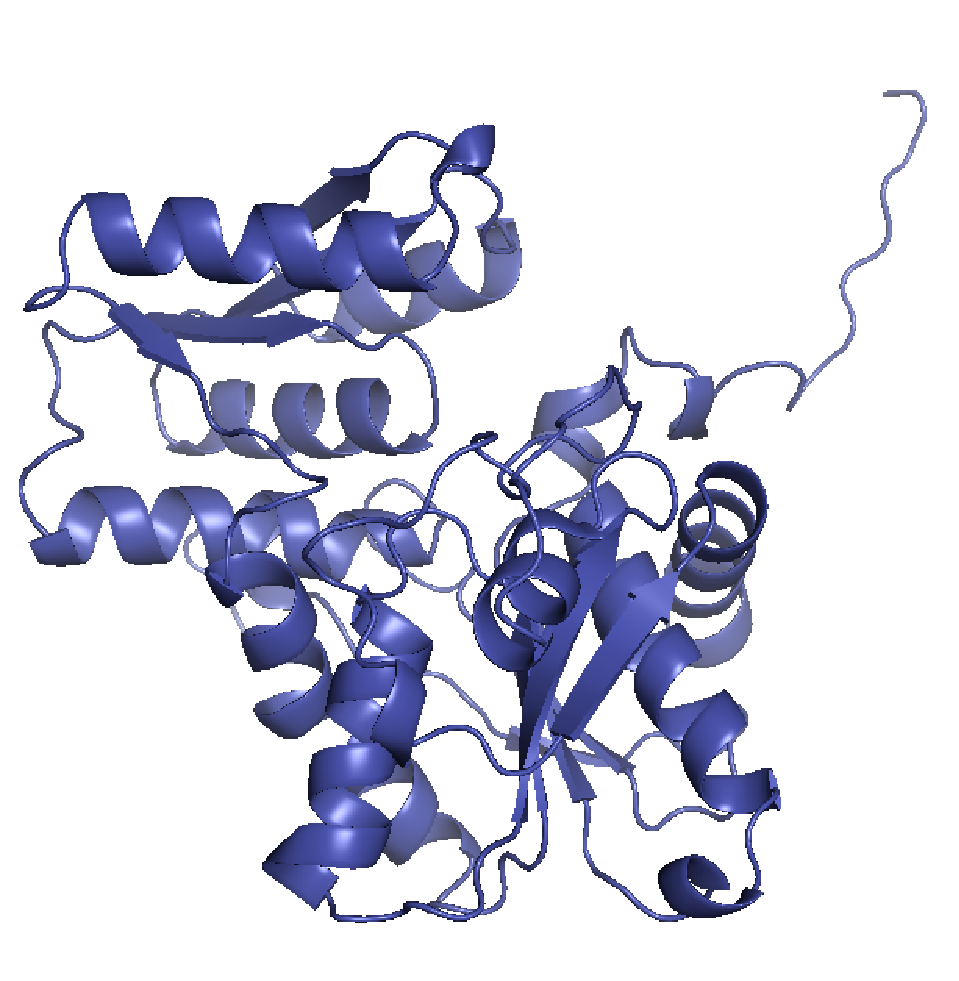
\includegraphics[scale=0.25]{model_T0861.pdf}}
	\captionof{figure}{Пример реальной и смоделированной структуры белка}
	\label{fig:edge}
\end{figure}
Белковая структура состоит из одной или нескольких цепочек более мелких молекул-- аминокислотных остатков. Последовательность остатков S = $\{a_i\}_{i=1}^N$ представляет его первичную структуру, где $a_i$ является одним из 22 типов аминокислот. Взаимодействия между соседними остатками и окружающей средой определяют, как цепочка будет сворачиваться в сложные структуры, которые представляют вторичную структуру и третичную структуру белка.

Поэтому для задач с участием белковых структур модель должна учитывать как пространственную информацию об атомах, третичную структуру, так и признаки в виде последовательностей аминокислот, первичную структуру белка.  В работах~\cite{HurtadoQA, AngularQA} для моделирования белков используются LSTM или 1D-CNN, которые представляют белки в виде последовательности с пространственными признаками.  В работах~\cite{3DCNN, 10.1093/bioinformatics/btz122} моделируется пространственная структура белков с использованием 3D-CNN, но не учитывается структура последовательностей. На основе графов моделируются как последовательности, так и геометрические структуры белков. 

В работе~\cite{Baldassarre2019GraphQAPM} графовые нейронные сети на основе алгоритма, описанного в~\cite{Battaglia2018RelationalIB}, показывают результаты, превосходящие остальные современные методы. Основные результаты в этой области полагаются на рточные нейронные сети (CNN)~\cite{10.1093/bioinformatics/btz122}. 

Поэтому предлагается использование графовых свёрточных нейронных сетей. 
%Кроме того, графы инвариантны к поворотам и сдвигам, может получать на вход белки разных размеров. 
%До недавнего времени лучшими методами предсказания стурктуры считались[?...?] объединение подходов, основанных на функциях, предназначенных для узкого класса белков. Методы глубинного обучения превзошли \cite{AlphaFold} эти результаты.
%Т.к. имеющиеся данные представляют собой трехмерные координаты атомов, то предлагается использовать графовые архитектуры нейронных сетей в комбинации с уже имеющимися архитектурами.

\section{Постановка задачи}

Пусть $\mathfrak{D} = \left\{\mathbf{x}_i, \mathbf{y}_i\right\}_{i=1}^m$~-- заданная выборка, где $\mathbf{X}\in \mathbb{R}^{m\times n\times 3}$~-- тензор объект-признак, объекты $\mathbf{x}_i\in \mathbb{R}^{1\times n_i\times 3}, i=\overline{1,m}$~-- это молекулы, каждая из которых описана множеством 3-мерных координат всех ее атомов, а $\mathbf{y} = [y_1,\dots, y_m]^{\mathsf{T}}\in \mathbb{R}^{m\times 1}$~-- оценка близости предсказанной и реальной структуры белка. Оценка близости измеряется различными метриками: $\text{CAD}_\text{score}$~\cite{Olechnovic2013CADscoreAN}, LDDT~\cite{Mariani2013lDDTAL}, GDT~\cite{GDT}. В данной работе выбран $\text{CAD}_\text{score}$. 

\subsection{CAD score}


%\begin{wrapfigure}{r}{0.32\textwidth}
%	\centering
%	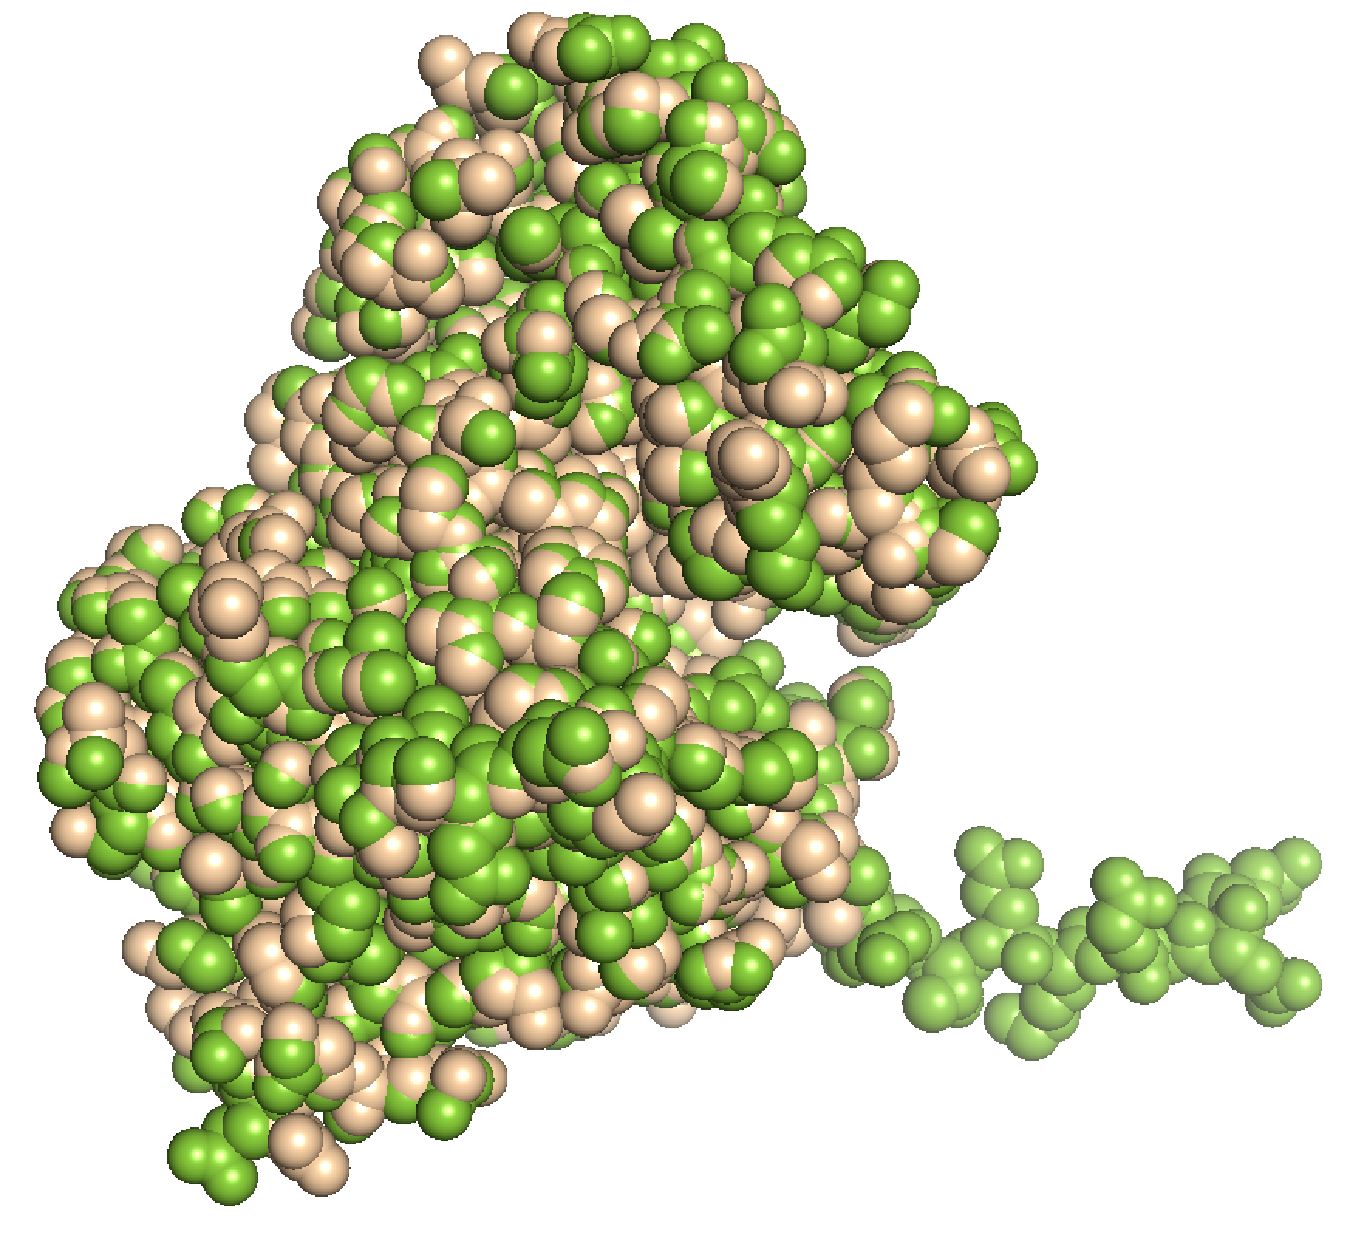
\includegraphics[width=0.3\textwidth]{T0861_Atome2_CBS_TS4.pdf}
%	\caption{Пересечение реальной и смоделированной структур}
%	\label{CAD_example}
%\end{wrapfigure}

Обозначим через $G$ множество всех пар элементов последовательности аминокислот (остатков)  $(i, j)$, имеющих ненулевую площадь контакта $T_{(i, j)}$ в реальной структуре. Затем для каждой пары остатков $(i, j)\in G$ вычисляется площадь контакта $M_{(i, j)}$ смоделированной структуры. 

Для каждой пары остатков $(i, j) \in G$ определяется разность площадей контакта $\mathrm{CAD}_{(i, j)}$ как абсолютная разница площадей контакта между остатками $i$ и $j$ в реальной $T$ и смоделированной структуре $M$:
$$\mathrm{CAD}_{(i, j)}=\left|T_{(i, j)}-M_{(i, j)}\right|.$$

Для вычислительной стабильности берется ограниченный CAD: $\mathrm{CAD}_{(i, j)}^{\text {bounded}}=\min \left(\mathrm{CAD}_{(i, j)}, T_{(i, j)}\right)$. Таким образом:
$\text{CAD}_\text{score}$для всей структуры определяется как
\begin{align}
\mathrm{CAD}_\text{score}=1-\cfrac{\sum_{(i, j) \in G} \mathrm{CAD}_{(i, j)}^{\text {bounded }}}{\sum_{(i, j) \in G} T_{(i, j)}}.
\label{CAD_score}
\end{align}

На рисунке~\ref{CAD_example} представлен пример пересечения реальной структуры T0861 (жёлтый) и её модели Atome2\textunderscore CBS\textunderscore TS4 (зелёный) при $\mathrm{CAD}_\text{score}=0.829$
\begin{figure}[h]
	\centering
	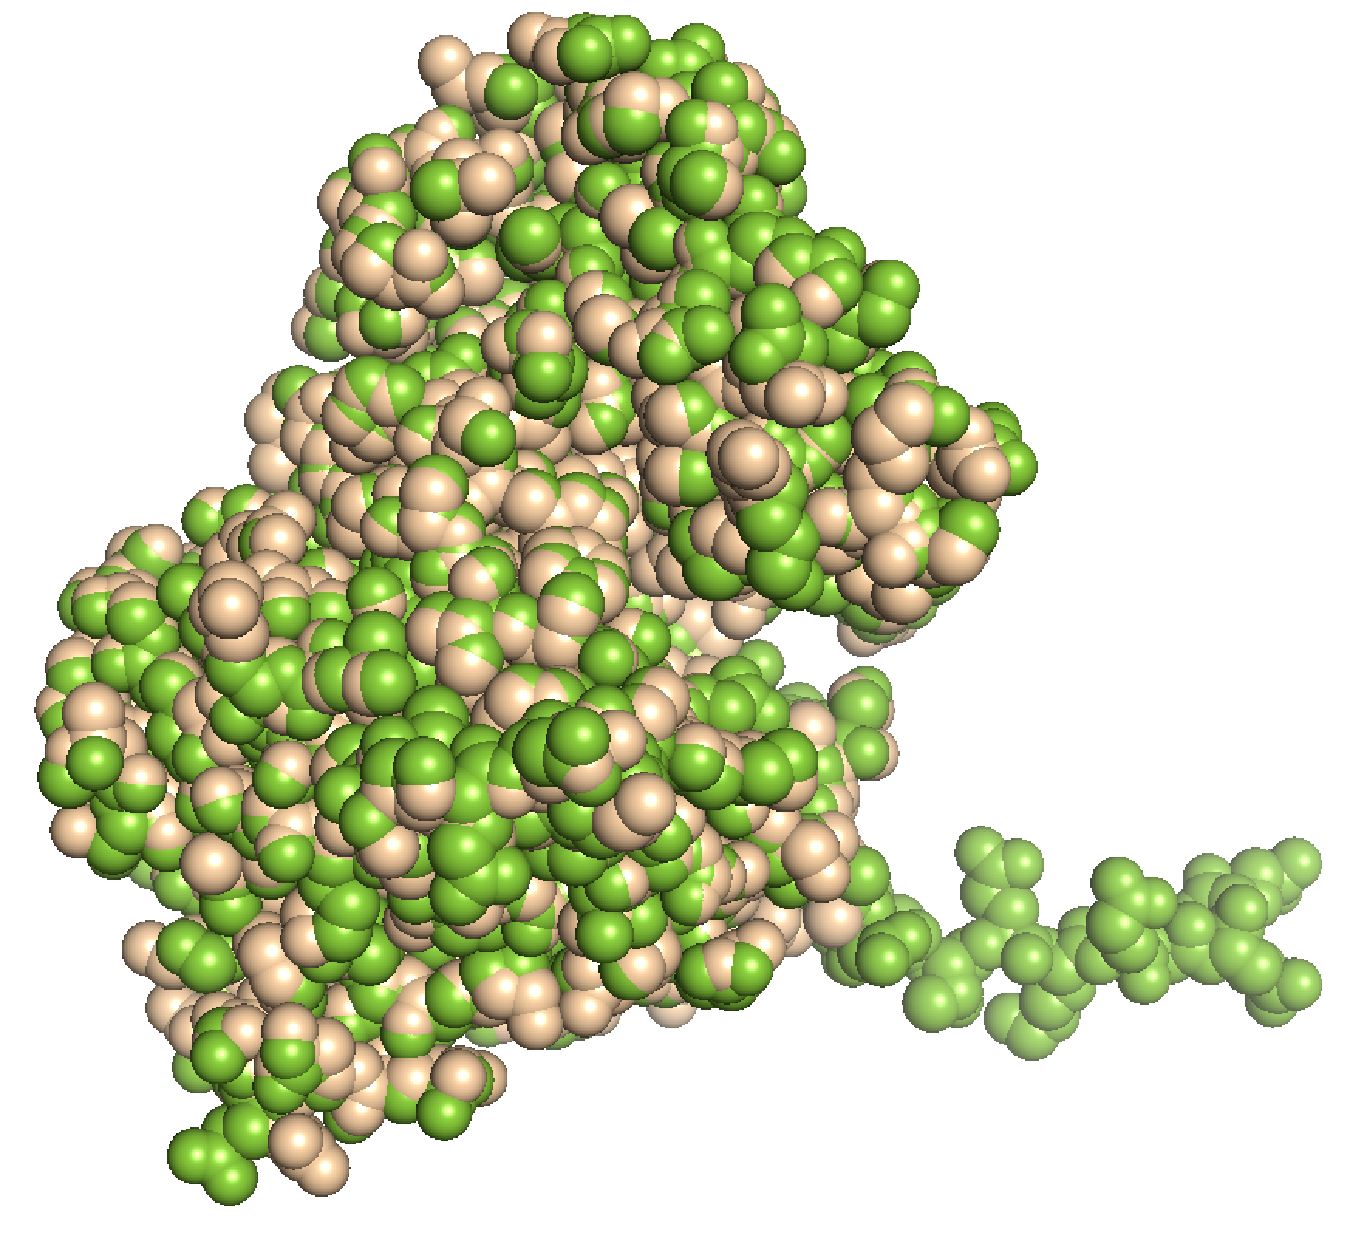
\includegraphics[width=0.3\textwidth]{T0861_Atome2_CBS_TS4.pdf}
	\caption{Пересечение реальной и смоделированной структур}
	\label{CAD_example}
\end{figure}
\subsection{Задача регрессии}

Рассмотривается множество параметрических моделей $\mathfrak{F}$, взятых из класса графовых свёрточных нейронных сетей: $\mathfrak{F} = \{\mathbf{f}_k\colon(\mathbf{w}, \mathbf{X})\to  \mathbf{\hat{y}}\mid k \in \mathfrak{K}\}$, где $\mathbf{w} \in \mathbb{W}$~-- параметры модели, а $\hat{\mathbf{y}}\in \mathbb{R}^{m\times 1}$~-- вектор оценок предсказаний CAD-scores. 

Решается задача регрессии для предсказания численного значения $\text{CAD}_\text{score}$ $y_i$ белка на основе его смоделированной пространственной структуры $\mathbf{x}_i$.

Параметры модели $\mathbf{w}\in \mathbb{W}$ подбираются в соответствии с минимизацией функции ошибки на обучении. Определим функцию ошибки
$\mathfrak{L}(\mathbf{y}, \mathbf{X}, \mathbf{w}) =\left( \mathbf{\hat{y}} - \mathbf{y} \right)^{2}$, где $\mathbf{\hat{y}} = \mathbf{f} (\mathbf{X},\mathbf{w})$-- $\text{CAD}_\text{score}$ предсказанный моделью $\mathbf{f}$, $\mathbf{y}$~-- данный в выборке $\text{CAD}_\text{score}$.
Т.е. решается данная задача оптимизации: 
$$\textbf{w}^* = \underset{\mathbf{w}\in\mathbb{W}}{\text{argmin}}(\mathfrak{L}(\textbf{w}))$$

Часто для оценивания модели используются коэффициенты корреляции Пирсона ($R$), Спирмена ($\rho$)~\cite{3DCNN, Baldassarre2019GraphQAPM, 10.1093/bioinformatics/btz122}. Для каждой реальной структуры белка вычисляются коэффициенты корреляции Пирсона ($R^{target}$), Спирмена ($\rho^{target}$) между истинными и прогнозируемыми $\text{CAD}_\text{score}$ для смоделированных структур, соответствующих данной реальной структуре белка. Затем коэффициенты корреляции усредняются по всем реальным структурам (m штук). Обозначим $\mathbf{y}_i$ и $\mathbf{\hat{y}}_i$ соответственно вектор истинных значений и вектор предсказаний $\text{CAD}_\text{score}$ для смоделированных структур белка, соответствующих реальной структуре $i$. Тогда коэффициенты корреляции записываются:
$$\begin{aligned}
R = R\left(\mathbf{y}, \hat{\mathbf{y}}\right) = \frac{1}{T} \sum_{i=1}^{T} R^\text{target}_i=\frac{1}{T} \sum_{i=1}^{T} \text{PEARSON} \left(\mathbf{y}_i,\hat{\mathbf{y}}_i\right) \\ 
\rho= \rho\left(\mathbf{y}, \hat{\mathbf{y}}\right) = \frac{1}{T} \sum_{i=1}^{T} \rho^\text{target}_i = \frac{1}{T} \sum_{i=1}^{T} \text{SPEARMAN} \left(\mathbf{y}_i,\hat{\mathbf{y}}_i\right)
\end{aligned}$$

$$r_{x y}=\frac{\sum_{i=1}^{m}\left(x_{i}-\bar{x}\right)\left(y_{i}-\bar{y}\right)}{\sqrt{\sum_{i=1}^{m}\left(x_{i}-\bar{x}\right)^{2} \sum_{i=1}^{m}\left(y_{i}-\bar{y}\right)^{2}}}$$
$$\hat{\rho}_{X_{1} X_{2}}=\frac{\sum_{i=1}^{n}\left(\operatorname{rank}\left(X_{1 i}\right)-\frac{n+1}{2}\right)\left(\operatorname{rank}\left(X_{2 i}\right)-\frac{n+1}{2}\right)}{\frac{1}{12}\left(n^{3}-n\right)}$$
\section{Спектральный анализ}

Для обобщения свёрточных нейронных сетей на графы необходимо определить свёрточные фильтры на графах. Существует два известных подхода: пространственный и спектральный~\cite{DBLP:journals/corr/abs-1901-00596, DBLP:journals/corr/abs-1812-08434}. Как показано в~\cite{ae482107de73461787258f805cf8f4ed} пространственный подход не имеет общего математического определения трансляции на графах, в то время как  спектральный метод имеет хорошее математическое обоснавание. Поэтому рассматривается спектральная теория графов.

%\subsection{Представление белков в виде графов}
Элементы аминокислотной последовательности рассматриваются как отдельные узлы, чьи связи (ребра) описывают пространственные отношения между ними. 

В общем случае граф $\mathbf{G}$ определяется набором $\mathbf{(V, A)}$, где $\mathbf{V}\in \mathbb{R}^{n \times c}$ определяет вершины или узлы графа. Матрица смежности $\mathbf{A}\in \mathbb{R}^{n \times n}$ определяет соединения между $n$ узлами (ребра), где $\mathbf{A}_{ij}$ – сила связи между узлами $i$ и $j$. Используя это определение графа, белковые структуры можно определить как графы, признаки элементов аминокислотной последовательности которых закодированы в элементах $\mathbf{V}$ узлов, а пространственная близость между элементами закодирована в матрице смежности $\mathbf{A}$.

\begin{Def}
	\textit{Графовый Лапласиан}~\cite{Chung:1997} -- матрица $\mathbf{L}=\mathbf{I}_{n}-\mathbf{D}^{-\frac{1}{2}} \mathbf{A} \mathbf{D}^{-\frac{1}{2}}$, где $\mathbf{A}$ -- матрица смежности графа $\mathbf{G}$,  $\mathbf{D}$ -- диагональная матрица степеней вершин, $\mathbf{D}_{i i}=\sum_{j}\left(\mathbf{A}_{i j}\right)$, $\mathbf{I}_{n}$-- единичная матрица.
\end{Def}

Матрица $\mathbf{L}$ является вещественной симметричной положительной полуопределенной, поэтому может быть представлена в виде  $\mathbf{L}=\mathbf{U} \boldsymbol{\Lambda} \mathbf{U}^{\mathsf{T}} $, где $\mathbf{U}=\left[\mathbf{u}_{\mathbf{0}}, \mathbf{u}_{\mathbf{1}}, \dots, \mathbf{u}_{\mathbf{n}-\mathbf{1}}\right] \in \mathbb{R}^{n \times n}$ -- это матрица собственных векторов, упорядоченных по собственным значениям, $\boldsymbol{\Lambda} \in \mathbb{R}^{n \times n}$~-- диагональная матрица собственных значений (спектр), $\boldsymbol{\Lambda}_{i i}=\lambda_{i}$. Спектральное разложение Лапласиана позволяет определить преобразование Фурье для графов: собственные векторы соответствуют модам Фурье, а собственные значения -- частотам. 

\begin{Def}
	\textit{Графовое преобразование Фурье}~\cite{journals/spm/ShumanNFOV13} для сигнала $\mathbf{x} \in \mathbb{R}^{n}$ задается $\mathscr{F}(\mathbf{x})=\mathbf{U}^{\mathsf{T}} \mathbf{x} \equiv \hat{\mathbf{x}} \in \mathbb{R}^{n}$, а обратное графовое пребразование Фурье: $\mathscr{F}^{-1}(\hat{\mathbf{x}})=\mathbf{U} \hat{\mathbf{x}}$, где $\mathbf{x}$ -- вектор признаков всех вершин.
\end{Def}

Данное преобразование является ключевым в определении графовой свёртки. Оно проецирует входной графовый сигнал на ортонормированное пространство, где базис формируется собственными векторами графового Лапласиана. Элементы преобразованного сигнала $ \hat{\mathbf{x}}$ являются координатами сигнала в новом пространстве, так что входной сигнал может быть представлен как $\mathbf{x}=\sum_{i} \hat{x}_{i} \mathbf{u}_{i}$, что является обратным графовым преобразованием Фурье.

\begin{Th}
	\textbf{(Теорема о свёртках)}~\cite{10.5555/1525499} Преобразование Фурье свёртки двух сигналов является покомпонентным произведением их преобразований Фурье, т.е. $$\mathscr{F}\left( \mathbf{f} * \mathbf{g}\right) =\mathscr{F}(\mathbf{f}) \odot \mathscr{F}(\mathbf{g})$$
	\label{conv_theorem}
\end{Th}

Следуя из теоремы~\ref{conv_theorem}, спектральная свёртка на графах определяется для сигнала $\mathbf{x}$ и фильтра $\mathbf{g} \in \mathbb{R}^{n}$ как 
\begin{align}
\mathbf{x} * \mathbf{g} &=\mathscr{F}^{-1}(\mathscr{F}(\mathbf{x}) \odot \mathscr{F}(\mathbf{g})) =\mathbf{U}\left(\mathbf{U}^{\mathsf{T}} \mathbf{x} \odot \mathbf{U}^{\mathsf{T}} \mathbf{g}\right) = \mathbf{U g}_{\theta} \mathbf{U}^{\mathsf{T}} \mathbf{x},\label{spec_conv}
\end{align}
где $\mathbf{g}_{\theta} = diag\left(\mathbf{U}^{\mathsf{T}} \mathbf{g}\right)$ -- спектральные коэффициенты фильтра.

Спектральные методы отличаются выбором фильтра $\mathbf{g}_{\theta}$. Соотношение \ref{spec_conv} вычислительно дорогое, т.к. спектральное разложение требует $O\left(n^{3}\right)$ операций, а перемножение с матрицей собственных векторов $\mathbf{U}$ требует $O\left(n^{2}\right)$ операций. Chebyshev Spectral CNN (ChebNet)~\cite{NIPS2016_6081} обходит эти проблемы аппроксимацией $\mathbf{g}_{\theta}$ с помощью полиномов Чебышева $\mathbf{T}_k\mathbf{(x)}$, убирая необходимость считать собственные векторы Лапласиана $\mathbf{L}$.

\begin{Def}
	\textit{Полиномы Чебышева} $\mathbf{T}_k\mathbf{(x)}$ $k$-ого порядка задаются рекуррентным соотношением  $ \mathbf{T}_{k}(\mathbf{x})=2 \mathbf{x} \cdot \mathbf{T}_{k-1}(\mathbf{x})-\mathbf{T}_{k-2}(\mathbf{x}), \mathbf{T}_{0}(\mathbf{x})=1, \mathbf{T}_{1}(\mathbf{x})=\mathbf{x}$. Образуют ортогональный базис в $L^{2}\left([-1,1], \cfrac{d x} {\sqrt{1-x^{2}}}\right)$
\end{Def}

Представляя $\mathbf{g}_{\theta}$ в виде 
\[\mathbf{g}_{\theta}=\sum_{k=0}^{K-1} \theta_{k} \mathbf{T}_{k}\mathbf{(\tilde{\Lambda})},	\]
где $\mathbf{\tilde{\Lambda}} = 2 \mathbf{\Lambda} / \lambda_{\max }-\mathbf{I}_{n} \in[-1,1]$, $\lambda_{\max }$ -- максимальное собственное число $\mathbf{L}$, а также замечая, что 
\[
\left(\mathbf{U} \mathbf{\Lambda} \mathbf{U}^{\mathsf{T}}\right)^{k}=\mathbf{U} \mathbf{\Lambda}^{k} \mathbf{U}^{\mathsf{T}}
\]
(собственные векторы образуют ортонормированный базис $\mathbf{U}^{\mathsf{T}}\mathbf{U}=\mathbf{I}$), получаем:
\begin{align}
\mathbf{U g}_{\theta} \mathbf{U}^{\mathsf{T}} \mathbf{x}=\mathbf{U}\left(\sum_{i=0}^{K-1} \theta_{k} \mathbf{T}_{k}(\tilde{\mathbf{\Lambda}})\right) \mathbf{U}^{\mathsf{T}} \mathbf{x} = \sum_{k=0}^{K-1} \theta_{k} \mathbf{T}_{k}(\tilde{\mathbf{L}}) \mathbf{x},
\label{cheb_appr}
\end{align}
где $\tilde{\mathbf{L}}=2 \mathbf{L} / \lambda_{\max }-\mathbf{I}_{n}$.

Graph Convolutional Network (GCN)~\cite{kipf_semi-supervised_2017} используют первое приближение ChebNet. Предполагая $\lambda_{\max} \approx 2$ и $K=1$, соотношение~\eqref{cheb_appr} упрощается до 
\begin{align}
\mathbf{x} * \mathbf{g} \approx \tilde{\theta}_{0} \mathbf{x}+\tilde{\theta}_{1}\left(\mathbf{L}-\mathbf{I}_{n}\right) \mathbf{x}=\tilde{\theta}_{0} \mathbf{x}-\tilde{\theta}_{1} \mathbf{D}^{-\frac{1}{2}} \mathbf{A} \mathbf{D}^{-\frac{1}{2}} \mathbf{x}.
\end{align}
Приняв $\theta = \tilde{\theta}_0  = -\tilde{\theta}_1$, получаем:
\begin{align}
\mathbf{x} * \mathbf{g}  \approx \theta\left(\mathbf{I}_{n}+\mathbf{D}^{-\frac{1}{2}} \mathbf{A} \mathbf{D}^{-\frac{1}{2}}\right) \mathbf{x}.
\label{conv}
\end{align}
Оператор в скобках может может привести к вычислительной нестабильности и взрыву или затуханию градиентов, т.к. собственные значения данного оператора $\in [0,2]$. Для решения проблемы в~\cite{kipf_semi-supervised_2017} предлагается \textit{трюк перенормировки}: 
\begin{align*}
\mathbf{I}_{n}+\mathbf{D}^{-\frac{1}{2}} \mathbf{A} \mathbf{D}^{-\frac{1}{2}} \rightarrow
\tilde{\mathbf{D}}^{-\frac{1}{2}} \tilde{\mathbf{A}}\tilde{\mathbf{D}}^{-\frac{1}{2}}, 
\text{ где }
\tilde{\mathbf{A}}=\mathbf{A}+\mathbf{I}_{n},~ \tilde{\mathbf{D}}_{i i}=\sum_{j} \tilde{\mathbf{A}}_{i j}.
\end{align*}
Дан граф $\mathbf{G}$ и матрица с информацией об узлах $\mathbf{X} \in \mathbb{R}^{n \times c}$ ($n$ -- число узлов и $c$ -- число признаков в каждом узле). Исходя из \eqref{conv} и применяя трюк перенормировки, определяется слой свёртки графа таким образом:
\begin{align}
\mathbf{Z}=\sigma\left(\tilde{\mathbf{D}}^{-\frac{1}{2}} \tilde{\mathbf{A}}\tilde{\mathbf{D}}^{-\frac{1}{2}} \mathbf{X} \mathbf{W}\right),
\label{Z_conv}
\end{align}
где $\mathbf{W} \in \mathbb{R}^{c \times t}$ – матрица параметров свёртки с $t$ фильтрами, $\sigma$ – нелинейная функция активации, а $\mathbf{Z} \in \mathbb{R}^{n \times t}$ -- выходная матрица.
\begin{figure}[h]
	\centering
	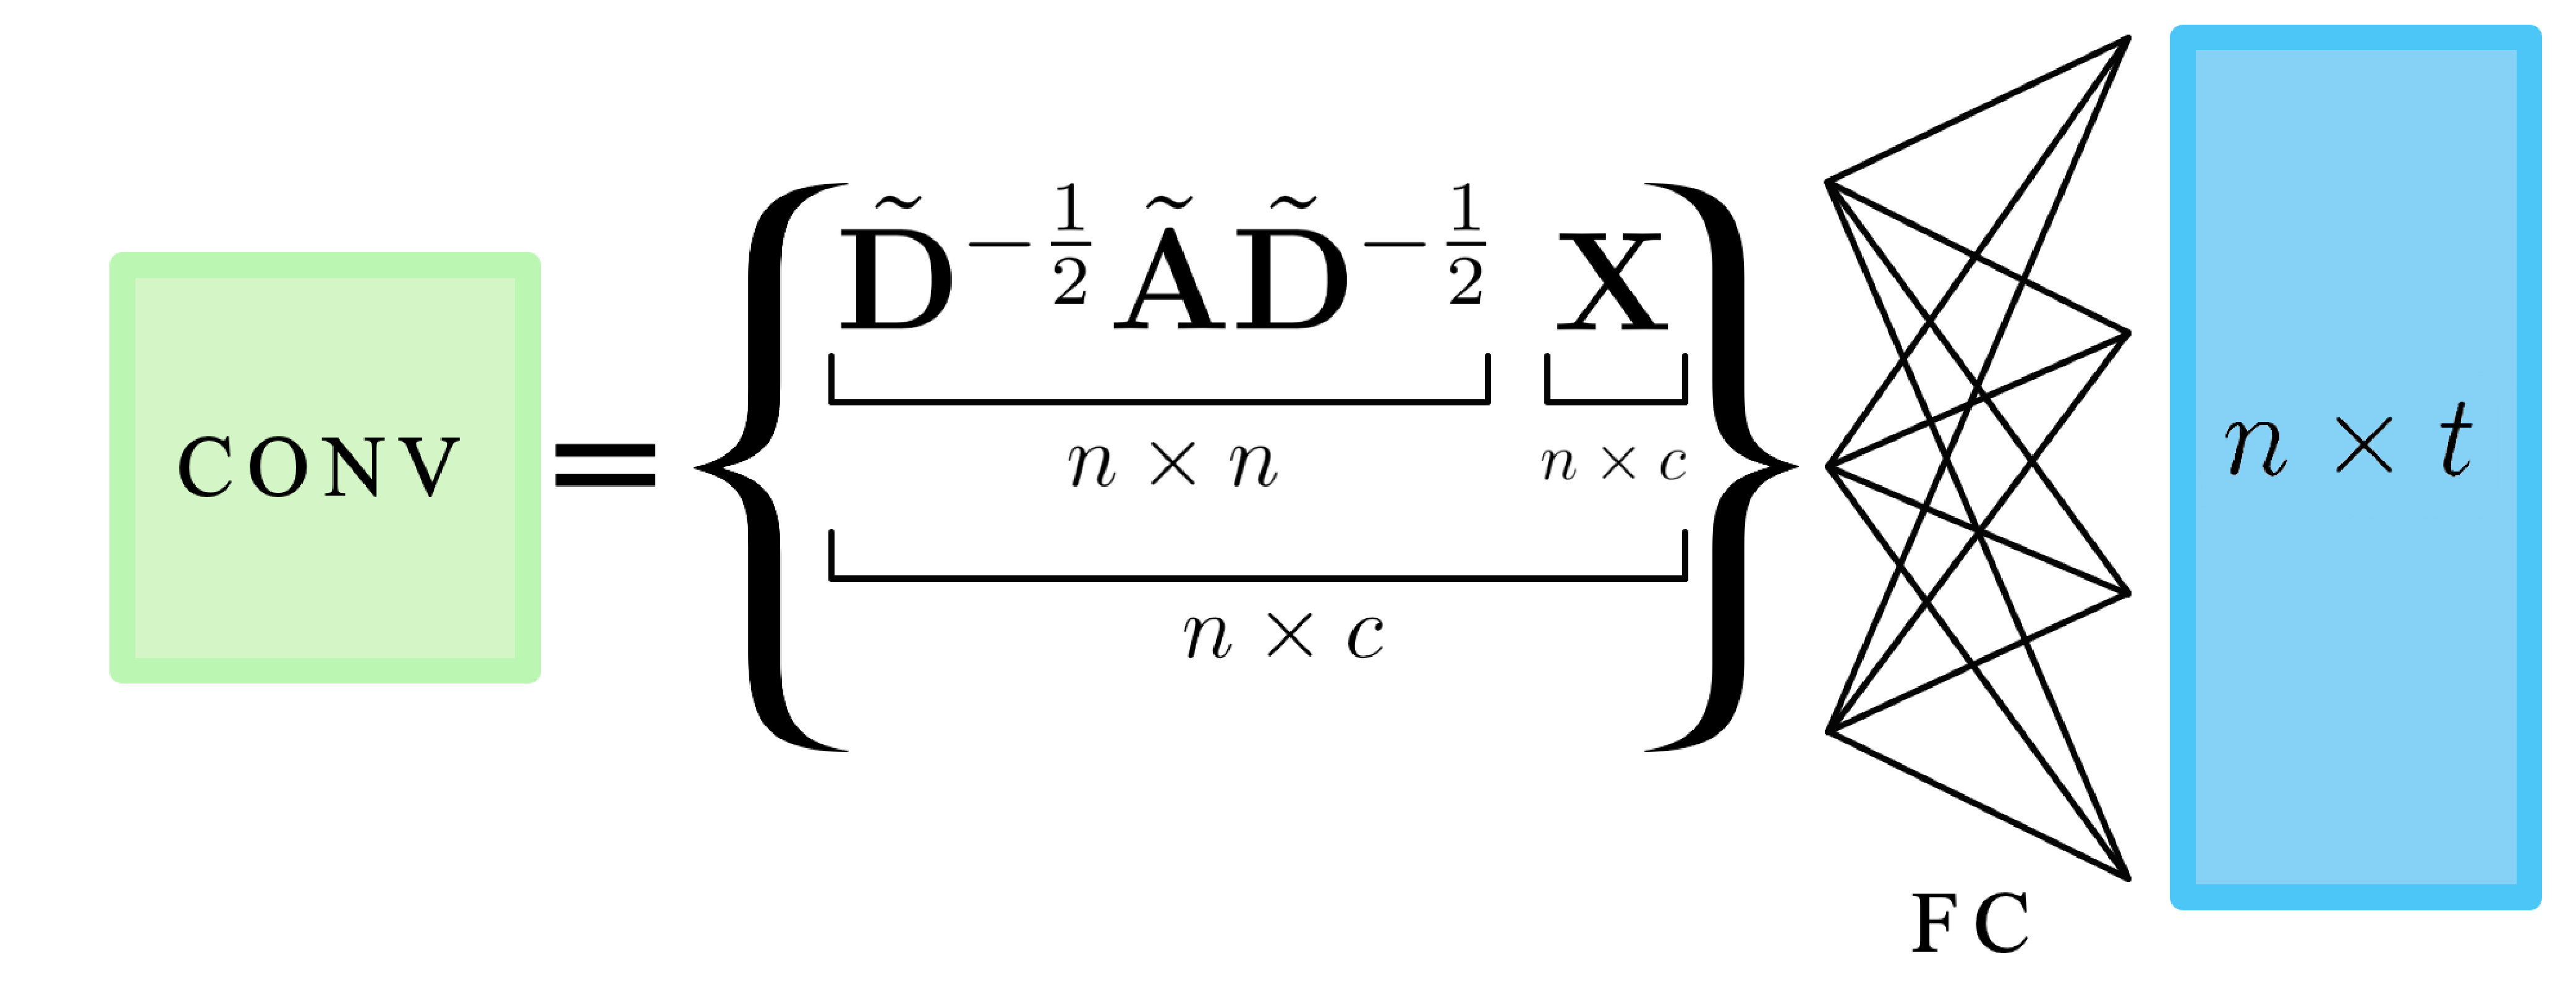
\includegraphics[width=0.9\textwidth]{conv_layer.pdf}
	\caption{Схема свёрточного слоя. $X$ -- подаваемая на вход слою матрица размера $n\times c$, $\text{t}$ -- количество фильтров в свёртке, FC -- полносвязный слой. Синий прямоугольник~-- выходная матрица размером $n\times t$}
	\label{fig:convlayer}
\end{figure}

\subsection{Архитектура сети}
Архитектура сети составляется по аналогии с моделью GCN~\cite{kipf_semi-supervised_2017}. На основе выражения~\eqref{Z_conv} определяются свёрточные слои (рисунок~\ref{fig:convlayer}). Нелинейная функция выбрана ReLu.

Сеть состоит из 3 свёрточных слоёв, макспуллинга по вершинам графа и нескольких полносвязных слоёв. Параметры свёрток $t$ взяты равными 64, 64, 64 соответственно для первого, второго, третьего свёрточных слоёв. На рисунке~\ref{fig:scheme} представлена схема тестируемой в работе нейронной сети.
\begin{figure}[h]
	\centering
	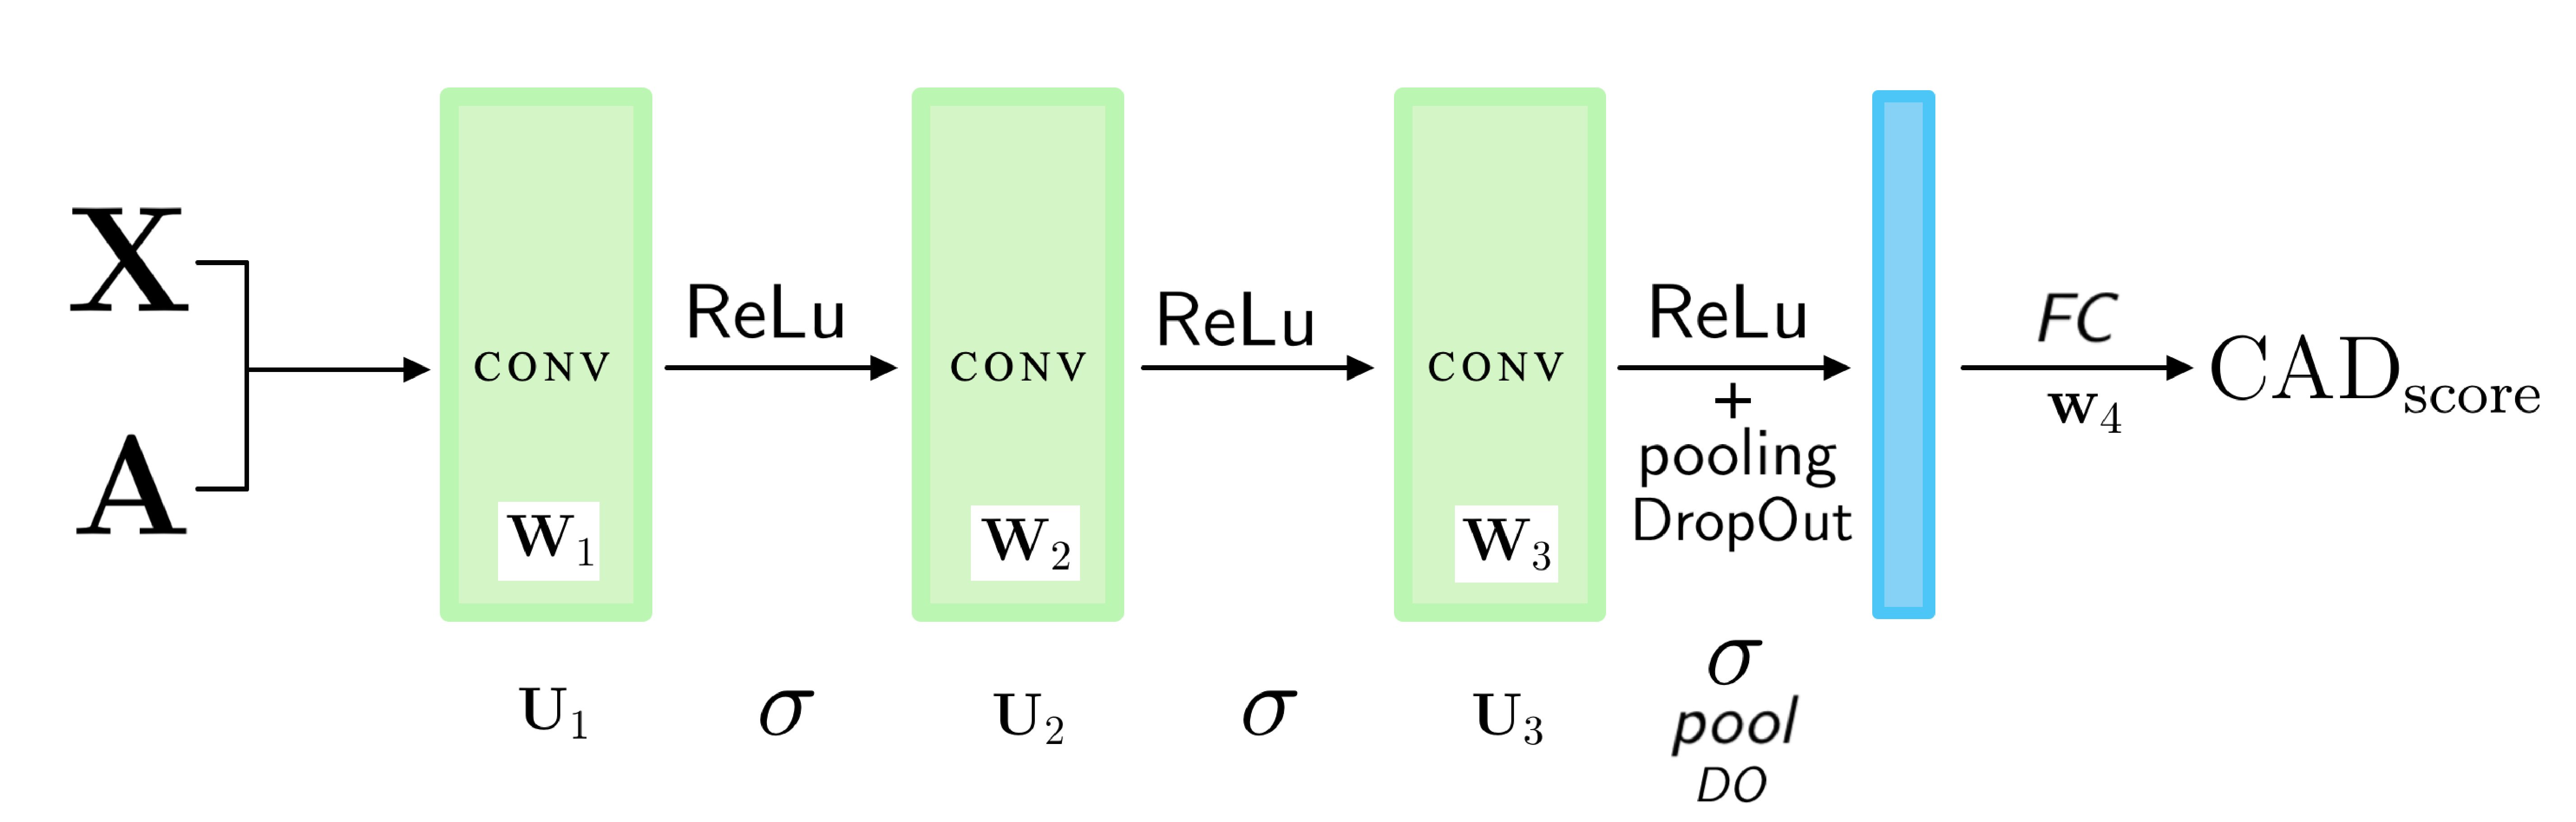
\includegraphics[width=0.99\textwidth]{net.pdf}
	\caption{Схематическое представление архитектуры свёрточной нейронной сети, использованной в данной работе}
	\label{fig:scheme}
\end{figure}
$$f = FC \circ DO \circ pool \circ \sigma \circ u_3\circ\sigma\circ u_2\circ\sigma\circ u_1$$
$$u_k = \tilde{\mathbf{D}}^{-\frac{1}{2}} \tilde{\mathbf{A}}\tilde{\mathbf{D}}^{-\frac{1}{2}} \mathbf{X} \mathbf{W}$$

\section{Вычислительный эксперимент}
Данные для эксперимента берутся с соревнований CASP разных лет. Используются наборы данных CASP7--CASP12 (таблица~\ref{table:student}). Обучение сети происходит на данных CASP7--CASP11 ($xxx$ таргетов, $xxxxx$ моделей), тестирование~-- на CASP12($xxx$ таргетов, $xxxxx$ моделей). Для процессов обучения и тестирования по формуле~\eqref{CAD_score} вычисляются $\text{CAD}_\text{score}$ для всех моделей структур на основе структур таргетов. 

\begin{table}[H]
		\centering
		\begin{tabular}{p{28mm}|p{26mm}p{26mm}|p{28mm}}
		\hline Набор & Реальные структуры & Модели структур& Разбиение\\
		\hline 
		CASP 7 & 95 & 24183 & \\
		CASP 8 & 123 & 36176 &  \multirow{2}{*}{Train,} \\
		CASP 9 & 117 & 35963 &  \multirow{2}{*}{Validation}\\
		CASP 10 & 103 & 15450 & \\
		CASP 11 & 84 & 12291 &  \\
		\hline 
		CASP 12 & 37 & 5538 & {Test} \\
		\hline
		Суммарно & 559 & 129601 &
		\end{tabular}
		\caption{Наборы данных}
		\label{table:student}
\end{table}

На рисунке~\ref{fig:experiment} представлена общая схема действий в эксперименте.

\begin{figure}[h]
	\centering
	\includegraphics[width=1.02\textwidth]{experiment.pdf}
	\caption{Общая схема эксперимента}
	\label{fig:experiment}
\end{figure}

\subsection{Матрица смежности}
Т.к. данные о белках не содержат информации о соединениях между атомами, т.е. нет матрицы смежности, для всех взятых моделей структур белков вычисляются матрицы смежности A по следующим правилам:
\begin{itemize}
	\item не соединяются водород с водородом,
	\item атом не соединяется с водородом, если расстояние между ними~$\geq 1.21$\AA,
	\item не соединяются атомы, которые находятся далеко в последовательности (номера остатков отличаются больше, чем на 1),
	\item не соединяются атомы, создающие дисульфидные связи,
	\item соединяются атомы, расстояние между которыми $r\in \left(r_\text{min}, r_\text{max}\right]$, где $r_\text{min} = 0.01$\AA, $r_\text{max} = \left(0.6\cdot(\rho_\text{atom1}+\rho_\text{atom2})\right)^2$, $\rho_\text{atom}$ -- радиус атома (максимально возможное $r_\text{max} = 5.76$ -- при $\rho_\text{atom1} = \rho_\text{atom2} = 2.0$).
\end{itemize}


\begin{figure}[H]
		\centering
		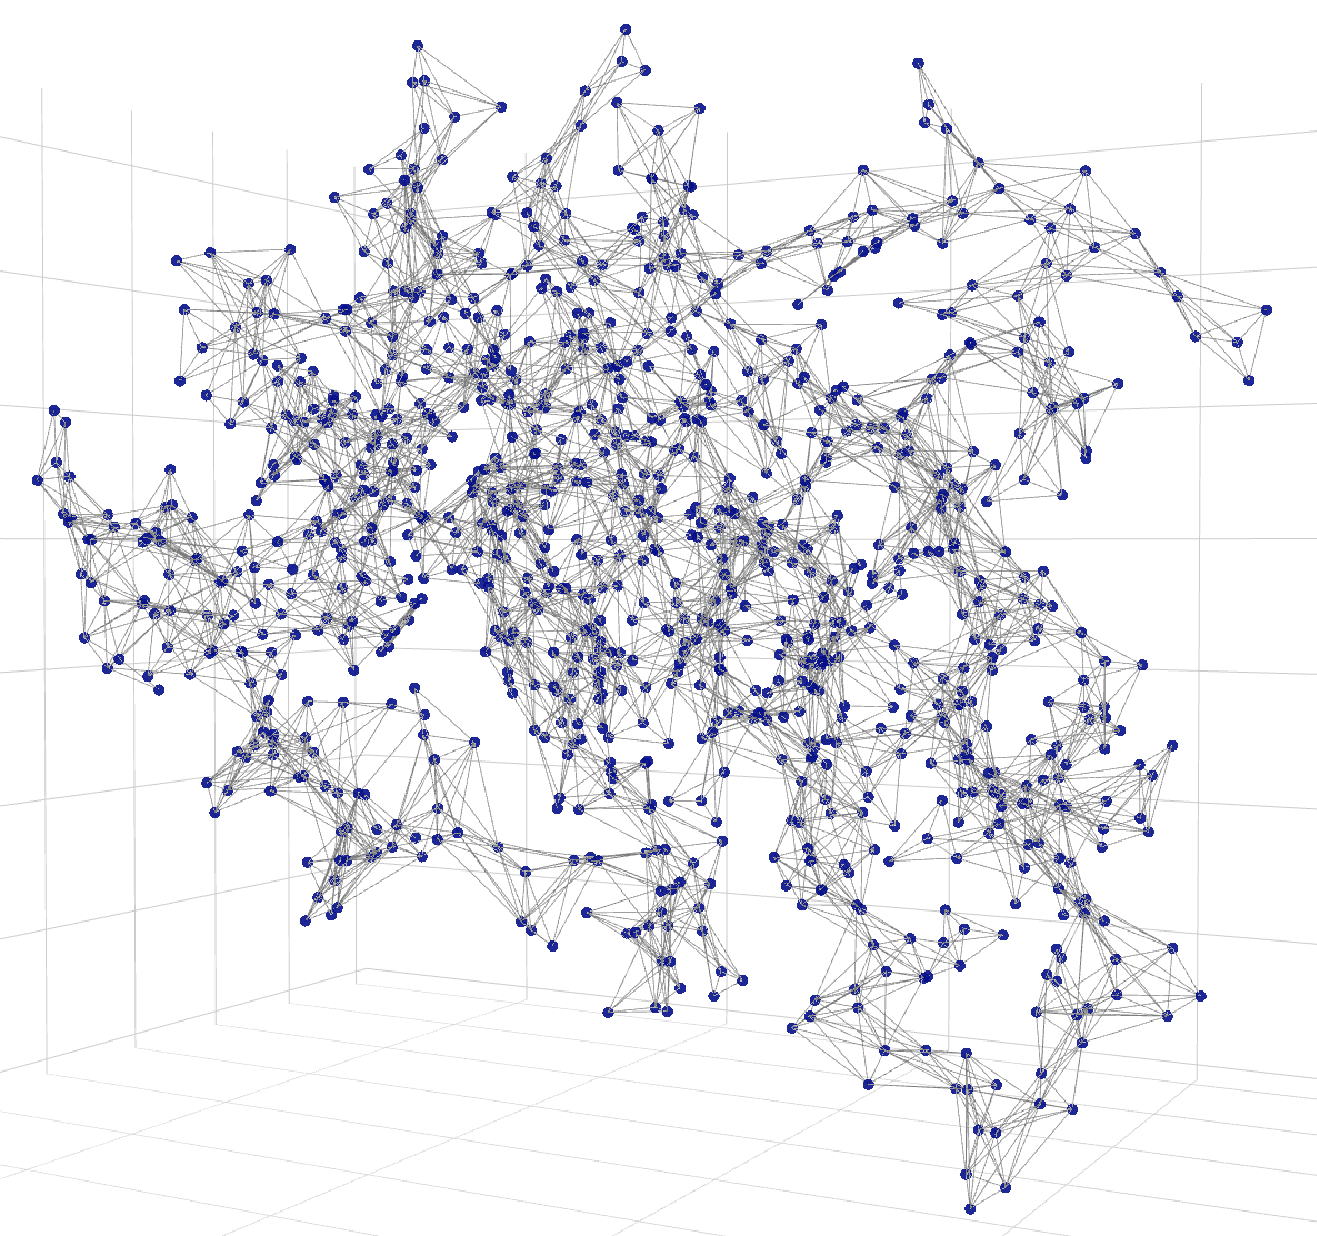
\includegraphics[width=0.7\textwidth]{3d_graph.pdf}
			\caption{Трехмерное представление с помощью координат и полученной матрицы смежности модели BAKER-ROSETTASERVER\_TS3 для таргета T0870 из набора данных CASP12}
			\label{fig:3Dgraph}
\end{figure}
	%\hfill
По попарным расстояниям между атомами на Рис. \ref{protein_vis} видно, что могут иметь соединения атомы, обозначенные самым светлым желтым, т.к. максимально возможное расстояние между атомами, при котором они могут иметь соединение по представленным правилам составления матрицы смежности равно 5.76 . Т.е. матрица смежности будет сильно разреженной.

	\begin{figure}[H]
		\centering
		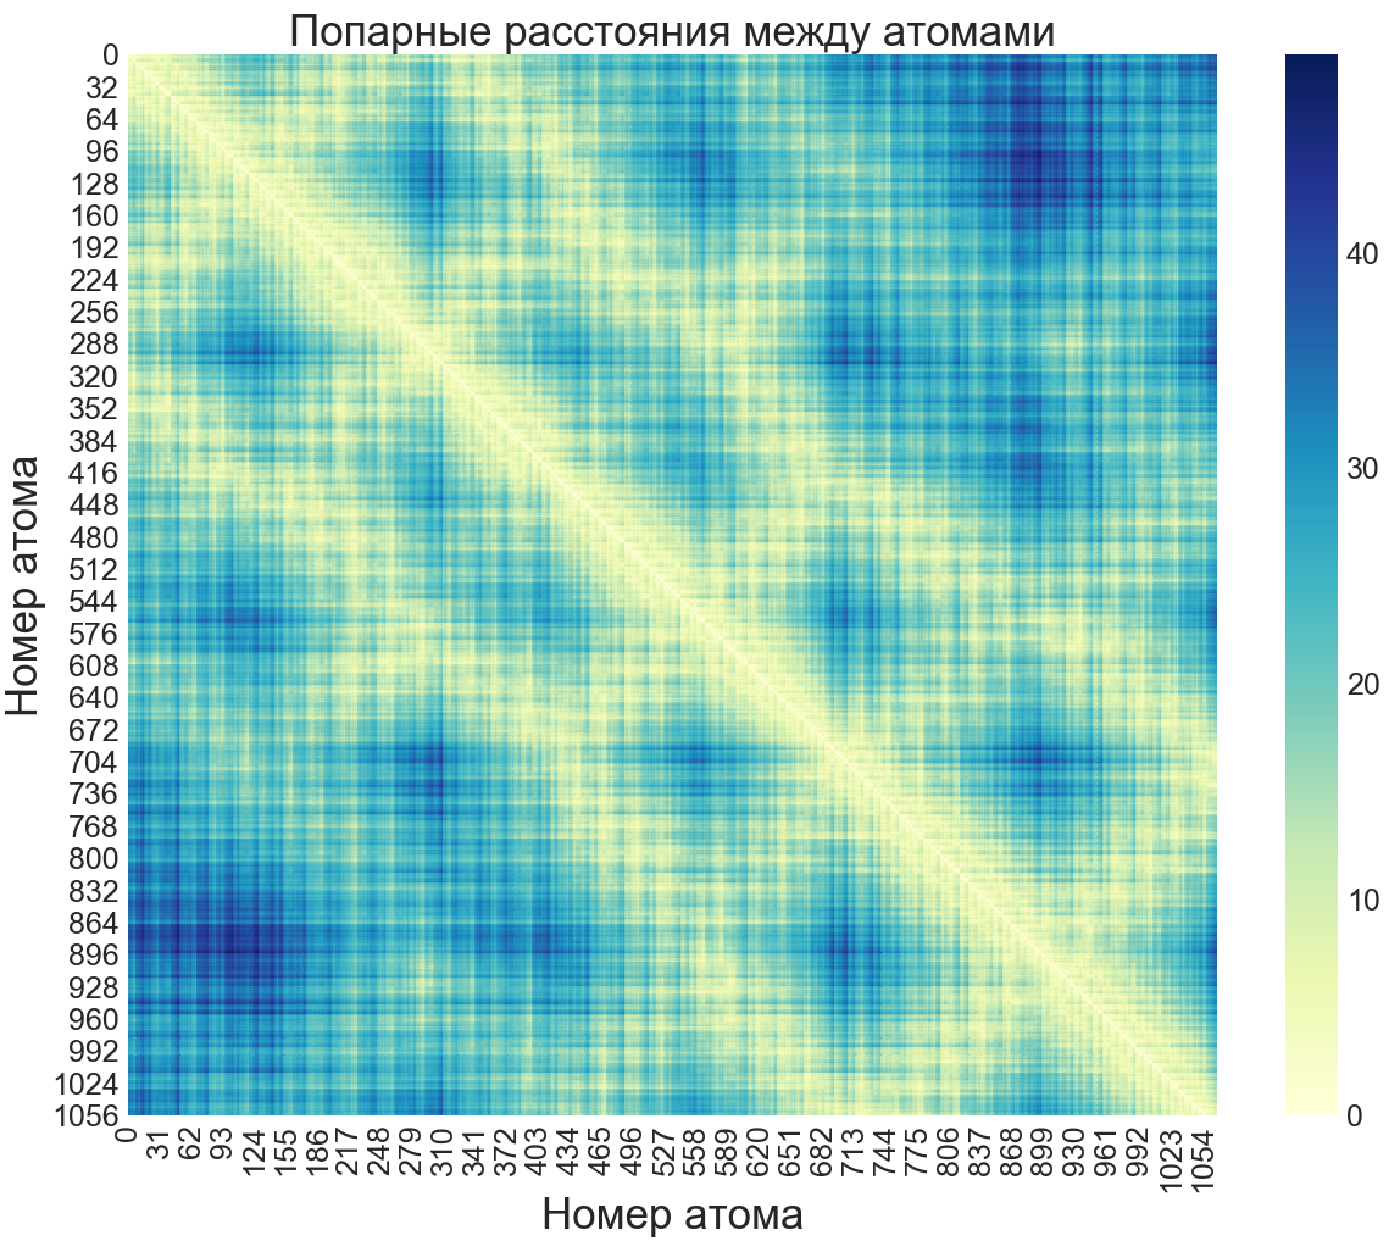
\includegraphics[width=0.8\textwidth]{pairwise.pdf}
		%	\caption{Попарные расстояния между элементами белка}
		%	\label{fig:data}
		\caption{попарные расстояния между атомами модели модели BAKER-ROSETTASERVER\_TS3 для таргета T0870 из набора данных CASP12}
		\label{protein_vis}
\end{figure}


\subsection{Собственное пространство матриц смежности}
Для каждой полученной матрицы смежности A производится сингулярное разложения для получения сингулярных чисел матрицы. Для оценки числа необходимых главных компонент матрицы используется правило сломанной трости.
\begin{figure}[H]
		\centering
		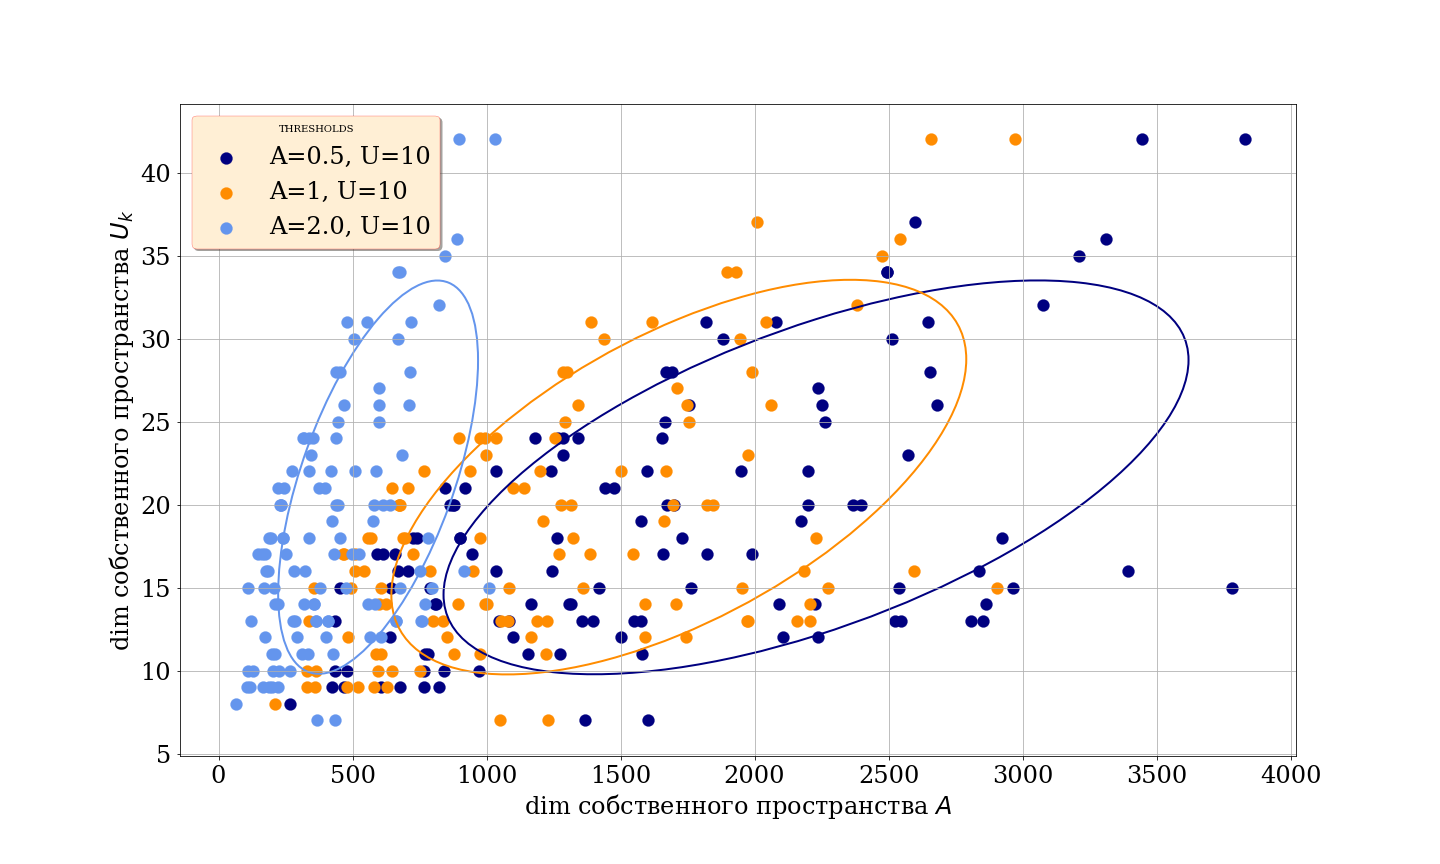
\includegraphics[width=0.8\textwidth]{eigens.pdf}
		\caption{Пример собственных чисел одной из матриц вместе с порогом 4}
		\label{fig:eigens}
\end{figure}
\begin{figure}[H]
		\centering
		\includegraphics[width=0.8\textwidth]{eigens_threshold.pdf}
		\caption{Количество собственных значений матриц, больших порога 4}
		\label{fig:threshold}
\end{figure}

\section{Результаты}
\begin{figure}[H]
		\centering
		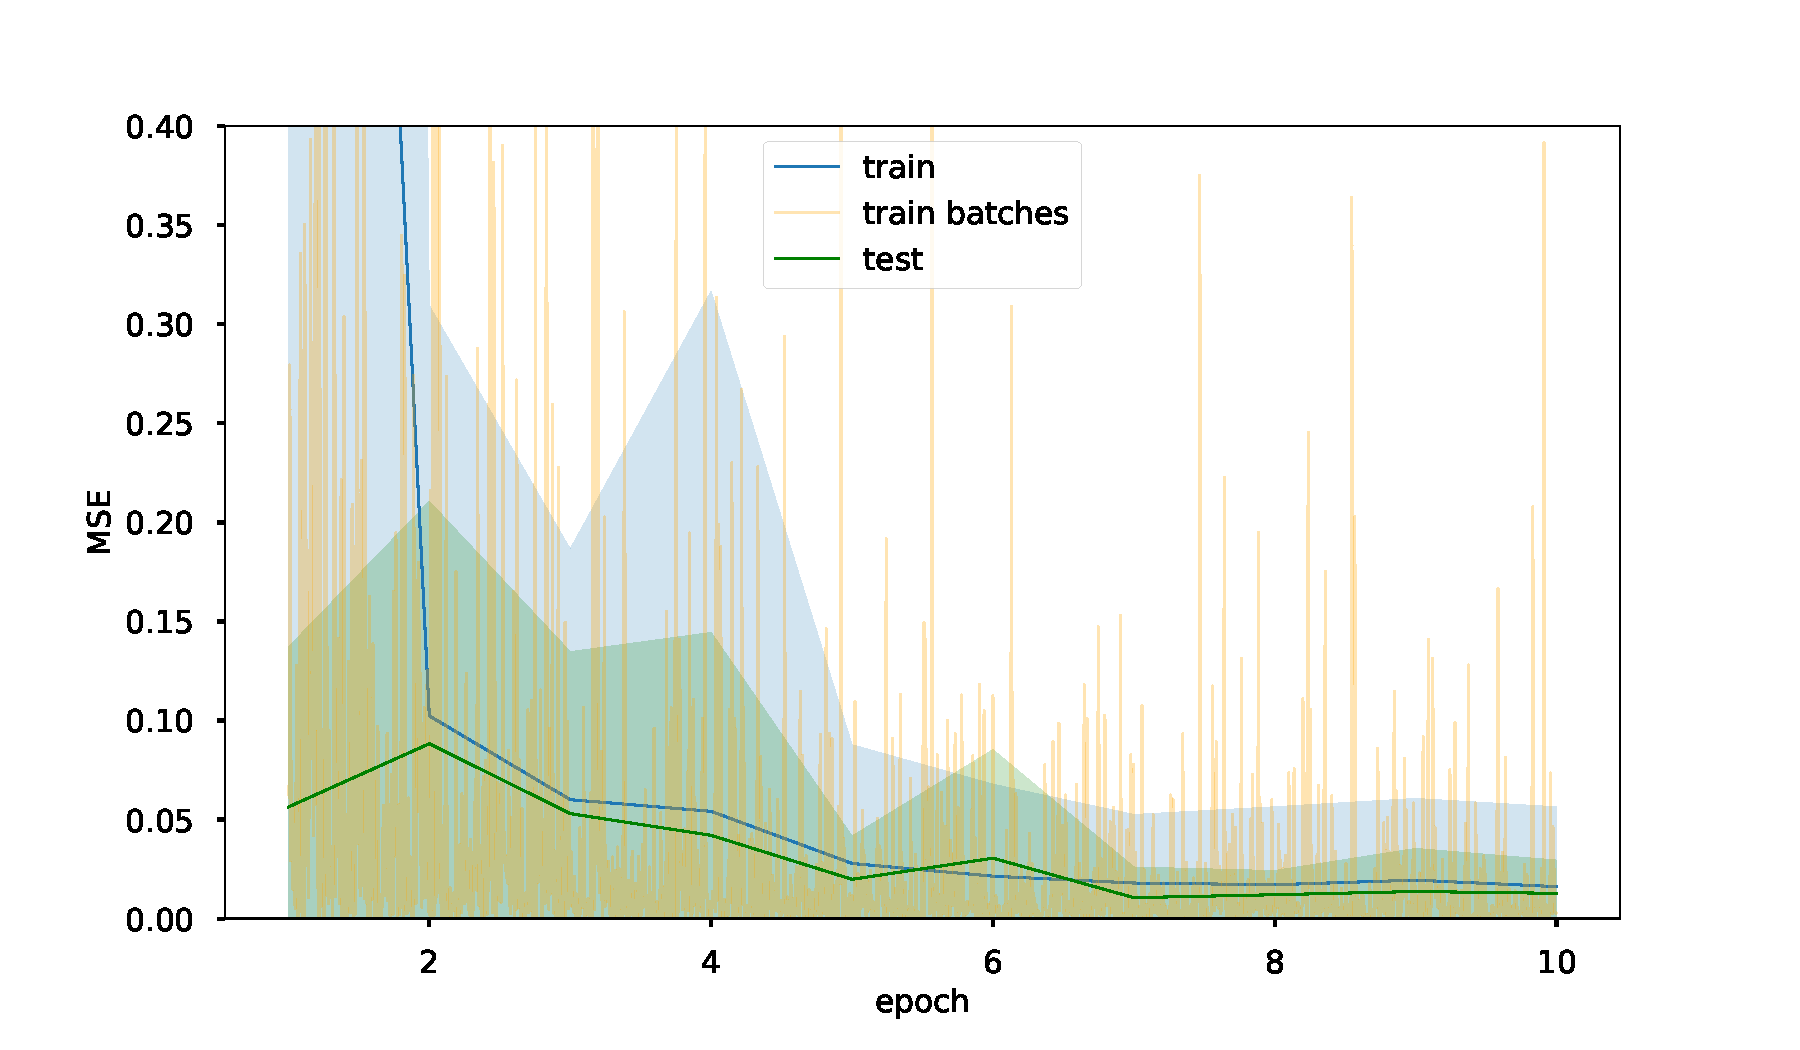
\includegraphics[width=0.8\textwidth]{training.pdf}
		\caption{График MSE ошибки GCN на обучающей и тестовой выборке}
		\label{fig:GCN}
	\end{figure}
\begin{figure}[H]
		\centering
		\includegraphics[width=0.55\textwidth]{training_correlations.pdf}
		\caption{Корреляция Пирсона, Кендалла, Спирмена}
		\label{fig:correlation}
\end{figure}

Сравнение с существующими методами QA:

\begin{center}
	\begin{table}[h]
		\centering
		%\begin{tabular}{l|l|l|l}
		\begin{tabular}{ccc}
			\hline Method & Spearmann $\rho$ &  Pearson $R$ \\
		\hline ProQ3D & 0.801 & 0.750 \\
		VoroMQA & 0.803 & 0.766  \\
		SBROD & 0.685 & 0.762  \\
		Ornate & 0.828 & 0.781   \\
		\textbf{SpectralQA} (МОЯ)&   \textbf{0}&   \textbf{0}    \\
		\hline 
		\end{tabular}
		\caption{Сравнение корреляции Пирсона, Спирмена и z-score существующих современных алгоритмов с моделью SpectralQA на данных CASP12}
		\label{Tab:1}
	\end{table}
\end{center}
***НЕСКОЛЬКО СЛОВ О РЕЗУЛЬТАТАХ ИЗ ТАБЛИЦЫ***



\section{Заключение}
Впервые для задачи оценки качества прогнозирования структуры белка применены графовые свёрточные нейронные сети, в которых свёртки определены на основе спектральной теории графов. В качестве улучшения, можно в основе архитектуры сети использовать другие существующие улучшения спектральных свёрток: CayleyNet, Adaptive Graph Convolution Network (AGCN), GRAPH WAVELET NEURAL NETWORK. Также предлагается учитывать в данных дополнительные химические свойства атомов и в матрице смежности учитывать не только наличие связи, но и расстояния между атомами при наличии связи.

\newpage




%%%%%%%%%%%%%%%%%%%%%%%%%%%%%%%%%%%%%%%%%%%%%%%%%%%%%%%%%%%%%%%%%%%%%%%%%
\newpage
\addcontentsline{toc}{section}{\protect\numberline{}Список литературы}
\bibliographystyle{ugost2008}
\bibliography{references}
\nocite{*}







\end{document} 